
\documentclass{bredelebeamer}
\usepackage{config}
%%%%%%%%%%%%%%%%%%%%%%%%%%%%%%%%%%%%%%%%%%%%%%%%

\title[Teoremas de tipo Bernstein--Doetsch]{
  Teoremas de tipo Bernstein--Doetsch para multifunciones 
  con terminos de error de tipo Takagi--Tabor.
}
% Titre du diaporama

\subtitle{Tesis Doctoral.}
% Sous-titre optionnel

\author [Carlos L. González.]{ 
  Autor: Carlos L. González. (UCV)\\
  Tutor: Dr. Nelson J. Merentes. (UCV) \\
  Co-tutor: Dr. Zsolt Páles. (UNIDEB)
}
% La commande \inst{...} Permet d'afficher l' affiliation de l'intervenant.
% Si il y a plusieurs intervenants: Marcel Dupont\inst{1}, Roger Durand\inst{2}
% Il suffit alors d'ajouter un autre institut sur le modèle ci-dessous.

%\today
% Optionnel. La date, généralement celle du jour de la conférence

\subject{math analysis convexity set-valued maps takagi transformation}
% C'est utilisé dans les métadonnes du PDF


\logo{
  
\includegraphics[scale=0.15]{images/SelloUCV.png}
}

%%%%%%%%%%%%%%%%%%%%%%%%%%%%%%%%%%%%%%%%%%%%%%%%%%%%%%%%%%%%%%%%%%%%%
\begin{document}

\begin{frame}
  \titlepage
\end{frame}

\begin{frame}{Contenido}
  \tableofcontents
  % possibilité d'ajouter l'option [pausesections]
\end{frame}




\section{Antecedentes}

\begin{frame}{Funciones convexas}
  
  \Defi{Convexidad}{
    Sea $f: [a,b]\to\R$ una funci\'on. Decimos que $f$ es \it{convexa}
    en $[a,b]$ sii, para todo $x,y\in[a,b]$ se tiene que 
    \Eq{convex}{
      f(tx + (1-t)y) \leq tf(x) + (1-t)f(y), \quad t\in[0,1].
    }
  }
    \begin{itemize}
    \item Premier point
    \end{itemize}
  \end{block}
Texte normal \alert{Texte Alert}  \exemple{Texte exemple} \emph{Texte emphase}

\begin{columns}

\begin{column}{0.5\textwidth}

\begin{exampleblock}{Bloc exemple}
\begin{itemize}
\item Premier point
\end{itemize}
\end{exampleblock}

\begin{alertblock}{Bloc alert}
\begin{itemize}
\item Premier point
\end{itemize}
\end{alertblock}

\end{column}

\begin{column}{0.5\textwidth}
\boiteviolette{
Une boite violette
}

\boiteorange{
Une boite orange
}

\boitegrise{
Une boite grise
}



\begin{tcolorbox}[tabvert,tabularx={X||Y|Y|Y|Y||Y}, boxrule=0.5pt, title=Mon tableau des prix]
Couleur & Prix 1  & Prix 2  & Prix 3 \\\hline\hline
Rouge   & 10.00   & 20.00   &  30.00 \\\hline
Vert    & 20.00   & 30.00   &  40.00  \\\hline
Bleu    & 30.00   & 40.00   &  50.00 \\\hline\hline
Orange  & 60.00   & 90.00   & 120.00 
\end{tcolorbox}

\end{column}

\end{columns}
\end{frame}




\section{Les blocs}

\begin{frame}{Les blocs}

\begin{block}{Bloc simple}
\begin{itemize}
\item Premier point
\item Second point
\item Troisième point
\end{itemize}
\end{block}

\begin{exampleblock}{Bloc exemple}
\begin{itemize}
\item Premier point
\item Second point
\item Troisième point
\end{itemize}
\end{exampleblock}

\begin{alertblock}{Bloc alert}
\begin{itemize}
\item Premier point
\item Second point
\item Troisième point
\end{itemize}
\end{alertblock}
\end{frame}


\section{Les bo\^ites}

\begin{frame}{Les boites}

\begin{columns}

\begin{column}{0.5\textwidth}
\boitejaune{
Ceci est \\
une boite jaune
}

\boiteorange{
Ceci est \\
une boite orange
}

\boitemarron{
Ceci est \\
une boite marron
}
\end{column}

\begin{column}{0.5\textwidth}
\boiteviolette{
Ceci est \\
une boite violette
}

\boitebleue{
Ceci est \\
une boite bleue
}

\boitegrise{
Ceci est \\
une boite grise
}

\end{column}

\end{columns}


\end{frame}



\section{Les listes}
	\subsection{Liste à item}

\begin{frame}{Titre de la frame}

	\begin{itemize}
		\item premier élément de liste,
		\item deuxième élément de liste,
		\item troisième élément de liste.
	\end{itemize}
\end{frame} 

		\subsection{Liste énumérative} 
\begin{frame}{Titre de la frame} 
	\begin{enumerate}
		\item élément de liste numéro 1,
		\item élément de liste numéro 2,
		\item élément de liste numéro 3.  
	\end{enumerate}
\end{frame}


		\subsection{Liste descriptive} 
\begin{frame}{Titre de la frame} 
	\begin{description}
		\item [Thème de présentation : ] ces thèmes sont en fait...
		\item [Thème de couleur : ] gère tout ce qui est couleur...
		\item [Thème de police : ] s'occupe de tout ce qui est police, gras...
		\item [Thème interne : ] s'occupe de l'apparence des éléments...
	\end{description}
\end{frame}



\section{Le texte}

\begin{frame}{Titre de la frame} 

Voici du texte normal

\alert{Voici du texte \texttt{alert}}

\exemple{Voici du texte \texttt{exemple}}

\emph{Voici du texte \texttt{emphase}}

\end{frame}


\section{Les tableaux}

\begin{frame}{Tableaux}

% merci: http://tex.stackexchange.com/questions/112343/beautiful-table-samples

\begin{tcolorbox}[tabjaune,tabularx={X||Y|Y|Y|Y||Y}, boxrule=0.5pt]
Couleur & Prix 1  & Prix 2  & Prix 3   & Prix 4   & Prix 5 \\\hline\hline
Rouge   & 10.00   & 20.00   &  30.00   &  40.00   & 100.00 \\\hline
Vert    & 20.00   & 30.00   &  40.00   &  50.00   & 140.00 \\\hline
Bleu    & 30.00   & 40.00   &  50.00   &  60.00   & 180.00 \\\hline\hline
Orange  & 60.00   & 90.00   & 120.00   & 150.00   & 420.00
\end{tcolorbox}

\begin{tcolorbox}[tabvert,tabularx={X||Y|Y|Y|Y||Y}, boxrule=0.5pt, title=Mon tableau des prix]
Couleur & Prix 1  & Prix 2  & Prix 3   & Prix 4   & Prix 5 \\\hline\hline
Rouge   & 10.00   & 20.00   &  30.00   &  40.00   & 100.00 \\\hline
Vert    & 20.00   & 30.00   &  40.00   &  50.00   & 140.00 \\\hline
Bleu    & 30.00   & 40.00   &  50.00   &  60.00   & 180.00 \\\hline\hline
Orange  & 60.00   & 90.00   & 120.00   & 150.00   & 420.00
\end{tcolorbox}

\end{frame}


\begin{frame}{Tableaux}

% merci: http://tex.stackexchange.com/questions/112343/beautiful-table-samples

\begin{tcolorbox}[tabgris,tabularx={X||Y|Y|Y|Y||Y}, boxrule=0.5pt]
Couleur & Prix 1  & Prix 2  & Prix 3   & Prix 4   & Prix 5 \\\hline\hline
Rouge   & 10.00   & 20.00   &  30.00   &  40.00   & 100.00 \\\hline
Vert    & 20.00   & 30.00   &  40.00   &  50.00   & 140.00 \\\hline
Bleu    & 30.00   & 40.00   &  50.00   &  60.00   & 180.00 \\\hline\hline
Orange  & 60.00   & 90.00   & 120.00   & 150.00   & 420.00
\end{tcolorbox}

\begin{tcolorbox}[taborange,tabularx={X||Y|Y|Y|Y||Y}, boxrule=0.5pt, title=Mon tableau des prix]
Couleur & Prix 1  & Prix 2  & Prix 3   & Prix 4   & Prix 5 \\\hline\hline
Rouge   & 10.00   & 20.00   &  30.00   &  40.00   & 100.00 \\\hline
Vert    & 20.00   & 30.00   &  40.00   &  50.00   & 140.00 \\\hline
Bleu    & 30.00   & 40.00   &  50.00   &  60.00   & 180.00 \\\hline\hline
Orange  & 60.00   & 90.00   & 120.00   & 150.00   & 420.00
\end{tcolorbox}

\end{frame}



\section{Les images}

\begin{frame}{Titre de la frame} 

\begin{figure}
\centering
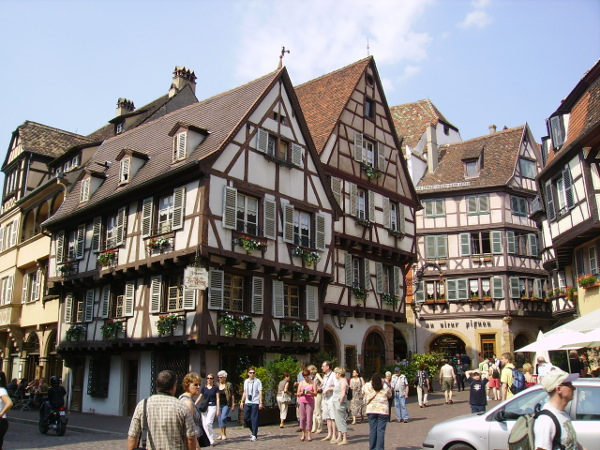
\includegraphics[scale=0.5]{images/architecturebretonne_wikipedia.jpg}
\caption{Éléments d'architecture bretonne typique du Sud de la France. (\href{http://commons.wikimedia.org/wiki/File:Colmar_-_Alsace.jpg}{Wikipédia.fr} CC-By-Sa)}
\end{figure}

\end{frame}



\end{document}
